\section{Introduzione}

\begin{domanda}
    (Cosa signifca costruire un classificatore?)

    Significa costruire una superficie di separazione. Per farlo si allena un
    modello utilizzando dei dati etichettati, che prende il nome di
    \textbf{training set}. Le superfici di separazione ci aiutano a classificare
    nuovi dati non visti.

    \textit{Esempio semplice}: chi paga il mutuo e chi no.
\end{domanda}

Una superficie di separazione è definita come:

$$ H(v,\gamma) = \{x \in \mathcal{R}^n | v^T x = \gamma\} $$
con:
\begin{itemize}
    \item $v \in R^n$ è un vettore, chiamato $normale$
    \item $\gamma \in R$ è uno scalare, che è il $bias$
\end{itemize}

La funzione \textbf{sign} ci dice da che parte del piano si trova un punto.
Cioè, dato un punto $\bar{x}$, se $sign(v^T \bar{x} - \gamma) \geq 0$ allora è
un cliente che paga il mutuo, altrimenti no.

\begin{domanda}
    (Dove interviene l'ottimizzazione quando si costruisce un classificatore? Perché serve?)

    Il classificatore viene costruito andando a \textbf{minimizzara} una misura che
    indica quanto si sta sbagliando nel classificare i punti.
\end{domanda}

\section{Programmazione non lineare}

\begin{definition}
    (Minimo globale)
    Dato un punto $x^* \in R^n$ si dice minimo globale se:
    \begin{itemize}
        \item $x^* \in X$, cioè il punto appartiene alla \textbf{regione ammissibile}
        \item $f(x^*) \leq f(x \forall x \in X)$, cioè per ogni punto della regione ammissibile, il valore di funzione obiettivo su $x^*$ è minore uguale rispetto agli altri punti.
    \end{itemize}
\end{definition}

\textbf{Notina:} Definizione di programma lineare:

\begin{itemize}
    \item $f(x) = c^T x$
    \item $X = \{x \in R^n | Ax = b, x \geq 0\}$
\end{itemize}
Dove $X$ è la regione ammissibile ed è un $poliedro$.

\begin{definition}
    (Minimo locale)

    Un punto $x^* \in X$ è un minimo locale per il problema $P$ se:
    \begin{itemize}
        \item $x^* \in X$
        \item Esiste un vicinato $N$ tale che $f(x^*) \leq f(x) \forall x \in X \cap N$. Cioé
              ogni punto della regione ammissibile intersecato col vicinato, e il valore
              $x^*$ è sempre minore.
    \end{itemize}
\end{definition}

Il vicinato è un insieme di punti, non so come definito ma ok.

\

\begin{definition}
    (Minimo locale stretto)

    Un punto $x^* \in X$ è un minimo locale stretto per il problema $P$ se:
    \begin{itemize}
        \item $x^* \in X$
        \item Esiste un vicinato $N$ tale che $f(x^*) < f(x) \forall x \neq x^*, x \in X \cap
                  N$.
    \end{itemize}
    Spiegazione al volo: Il minimo locale stretto è un minimo locale, ma non esistono altri punti che hanno lo stesso valore di funzione obiettivo.

    \begin{figure}[H]
        \centering
        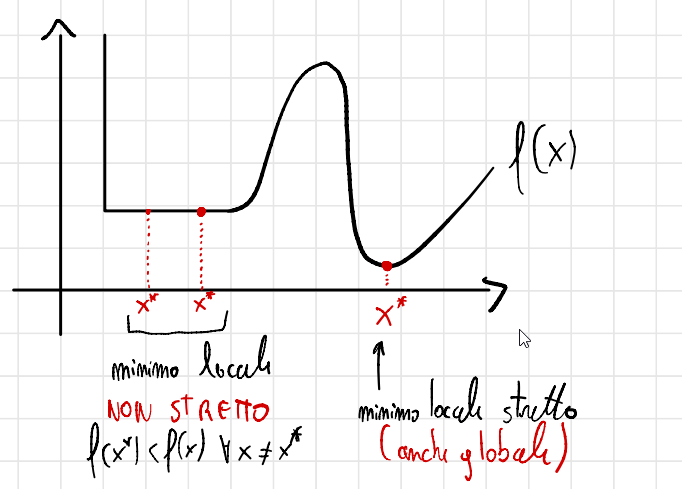
\includegraphics[width=0.8\textwidth]{images/minimo locale.png}
        \caption{Esempio di minimo locale stretto}
        \label{fig:esempio-di-minimo-locale-stretto}
    \end{figure}
\end{definition}

\textbf{Nota:} Se $x^*$ è un minomo globale implica che $x^*$ è un minimo locale.

\begin{definition}
    (Combinazione convessa)

    Dati $x^{(1)}$ e $x^{(2)}$ due punti $\in R^n$, la combinazione convessa di
    $x^{(1)}$ e $x^{(2)}$ è un vettore:

    $$
        \bar{x} = \lambda x^{(1)} + (1 - \lambda) x^{(2)}$$
    con $\lambda \in [0,1]$

    Immagina una retta che unisce i due punti, con $\lambda$ = 0 in $x^{(1)}$ e
    $\lambda$ = 1 in $x^{(2)}$.
\end{definition}

\begin{definition}
    (Funzione convessa)

    Data una funzione $f: R^n \rightarrow R$, $f$ è \textbf{convessa} se per ogni
    coppia di punti $x^{(1)}, x^{(2)} \in R^n$ e per ogni $\lambda \in [0,1]$ vale
    che: $$ f(\lambda x^{(1)} + (1 - \lambda) x^{(2)}) \leq \lambda f(x^{(1)}) + (1
        - \lambda) f(x^{(2)}) $$

    Cioè in italiano, il valore di funzione della combinazione dei due vettori è
    minore o uguale alla combinazione dei valori di funzione dei due vettori.

    \begin{figure}[H]
        \centering
        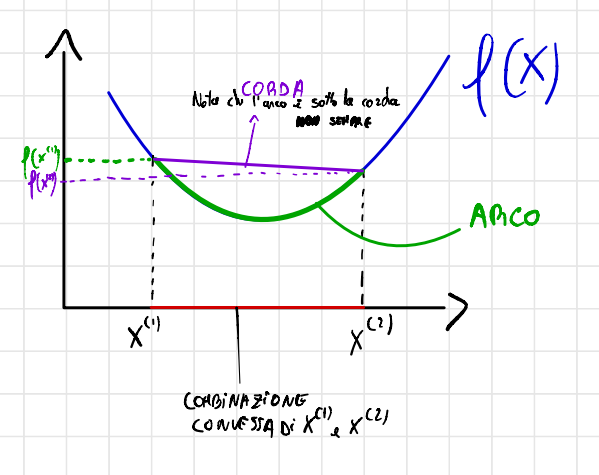
\includegraphics[width=0.8\textwidth]{images/funz conv.png}
        \caption{Esempio di funzione convessa}
        \label{fig:esempio-di-funzione-convessa}
    \end{figure}

    \begin{figure}[H]
        \centering
        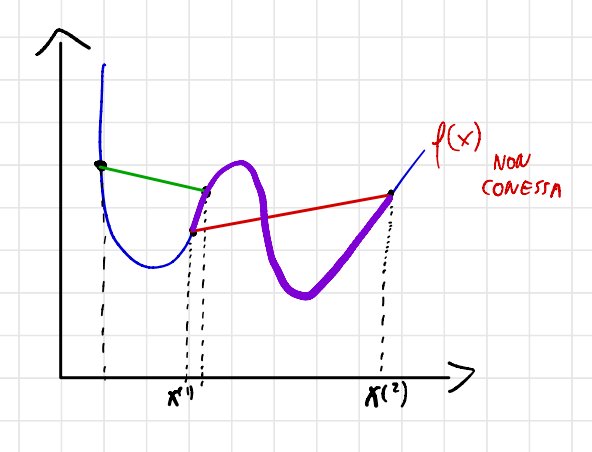
\includegraphics[width=0.8\textwidth]{images/non conv.png}
        \caption{Esempio di funzione non convessa}
        \label{fig:esempio-di-funzione-non-convessa}
    \end{figure}

    Per capire, diciamo che la funzione è convessa se per ogni valore di funzione
    su un punto che è all'interno della combinazione convessa dei due punti, il
    valore di funzione è minore o uguale alla combinazione dei valori di funzione
    dei due punti.

    Infatti, nel secondo esempio, ci sono dei punti tali per cui la funzione è
    maggiore (cioè sta sopra).
\end{definition}

\begin{domanda}
    (Quando un punto di un'insieme convesso è estremo?)

    $\bar{x} \in X$ è un punto estremo di un'insieme convesso se NON ESISTE nessuna coppia di punti $x^{(1)}, x^{(2)} \in X$ e $\lambda \in (0,1)$ tale che:
    $\bar{x} = \lambda x^{(1)} + (1 - \lambda) x^{(2)}$, per $\lambda \in ]0,1[$.

    Banalmente, un punto è estremo se non è combinazione convessa di altri punti.
\end{domanda}

\textbf{Nota:} $P$ è un programma convesso se $f$ è una funzioen convessa e $X$ è un'insieme convesso. Questo ci serve saperlo perché in caso di
\textbf{programma convesso} abbiamo che il minimo globale e locale \textbf{coincidono}.

\begin{domanda}
    (Cosa cerchiamo con un problema di ottimizzazione?)

    Cerchiamo il \textbf{minimo locale}, perché cercare il minimo globale fa parte
    di un'altra categoria di problemi, che sono quelli di \textbf{ottimizzazione
        globale}.
\end{domanda}

\subsubsection{Caso di problemi senza vincoli}

In questo caso, la regione ammissibile $X$ coincide con $R^n$.

$$
    P = \begin{cases}
        \min f(x) \\
        f(x): \mathcal{R}^n \rightarrow R
    \end{cases}
$$

\textbf{Nota:} Si fa un'assunzione. $f \in C^2$, cioè la funzioen è due volte
continuamente differenziabile. Quindi, $C^2$ è l'insieme di funzioni che ammettono prima e seconda derivate continue.

Questa assunzione ci permette di dire che $\bar{x} \in R^n \implies \nabla f(\bar{x})$ e $\nabla^2 f(\bar{x})$ esistono.


Vediamo come si applica il gradiente e la matrice hessiana.

\begin{definition}
    (Gradiente)

    Il gradiente di una funzione $f: R^n \rightarrow R$ è un vettore di dimensione
    $n$ che contiene le derivate parziali della funzione rispetto alle sue
    variabili.

    $$
        \nabla f(x) = \begin{bmatrix}
            \frac{\partial f}{\partial x_1} \\
            \frac{\partial f}{\partial x_2} \\
            \vdots                             \\
            \frac{\partial f}{\partial x_n}
        \end{bmatrix}
    $$
\end{definition}

\begin{definition}
    (Matrice Hessiana)

    La matrice hessiana di una funzione $f: R^n \rightarrow R$ è una matrice
    quadrata di dimensione $n$ che contiene le derivate seconde parziali della
    funzione rispetto alle sue variabili.

    $$
        \nabla^2 f(x) = \begin{bmatrix}
            \frac{\partial^2 f}{\partial x_1^2} & \frac{\partial^2 f}{\partial x_1 \partial x_2} & \dots  & \frac{\partial^2 f}{\partial x_1 \partial x_n} \\
            \frac{\partial^2 f}{\partial x_2 \partial x_1} & \frac{\partial^2 f}{\partial x_2^2} & \dots  & \frac{\partial^2 f}{\partial x_2 \partial x_n} \\
            \vdots & \vdots & \ddots & \vdots \\
            \frac{\partial^2 f}{\partial x_n \partial x_1} & \frac{\partial^2 f}{\partial x_n \partial x_2} & \dots  & \frac{\partial^2 f}{\partial x_n^2}
        \end{bmatrix}
    $$
\end{definition}

\begin{esempio}
    f(x) = $8x_1 + 12x_2 + x_1^2 - 2x_2^2$

    Iniziamo dal gradiente.

    $$
        \nabla f(x) = \begin{bmatrix}
            8 +2x_1 \\
            12 - 4x_2
        \end{bmatrix}
    $$

    Ora la matrice hessiana.

    $$
        \nabla^2 f(x) = \begin{bmatrix}
            2 & 0  \\
            0 & -4
        \end{bmatrix}
    $$
    
    Dando un valore ad $x$, ad esempio $x = \begin{bmatrix}
        1 \\
        1
    \end{bmatrix}$, possiamo calcolare il gradiente e la matrice hessiana cosi:

    $$
        \nabla f(x) = \begin{bmatrix}
            10 \\
            8
        \end{bmatrix}
    $$

    $$
        \nabla^2 f(x) = \begin{bmatrix}
            2 & 0  \\
            0 & -4
        \end{bmatrix}
    $$
\end{esempio}

\subsection{Condizioni di ottimalità}
Sono 3

\begin{definition}
    (Prima condizione - condizione necessaria di primo ordine)
    $x^*$ è un minimo locale implica che $\implies \nabla f(x^*) = 0$. Cioè,
    stiamo dicendo che $x^*$ è un punto stazionario. Il fatto che 
    il gradiente sia uguale a 0 è una condizione necessaria per fare in modo che 
    $x^*$ sia un minimo locale.

    \textbf{Nota:} Se $f$ è convessa, allora ogni punto stazionario è 
    un \textbf{minimo globale}.
    (Pensa ad una funzione che è convessa ma ha più punti di minimo uguali)
\end{definition}

\begin{definition}
    (Seconda condizione - condizione necessaria di secondo ordine)
    $x^*$ è un minimo locale stretto $\implies \nabla f(x^*) = 0$ e 
    $\nabla^2 f(x^*)$ è  positiva semidefinita. Lo definiamo dopo cosa Significa
    positiva semidefinita
\end{definition}

\begin{definition}
    (Terza condizione - condizione sufficiente di secondo ordine)
    Sia $x^* \in R^n$, sia $\nabla f(x^*) = 0$ e $\nabla^2 f(x^*)$ 
    positiva definita $\implies x^*$ è un \textbf{minimo locale stretto}.
\end{definition}

Definiamo cosa significa semidefinita ecc.

Sia $A$ una matrice $R^{n \times m}$:
\begin{itemize}
    \item \textbf{Positiva Semidefinita}: $\forall x \in R^n, x^TAx \geq 0$
    \item \textbf{Positiva Definita}: $\forall x \in R^n, x^TAx > 0$, con $x \neq 0$
    \item \textbf{Negativa Semidefinita}: $\forall x \in R^n, x^TAx \leq 0$
    \item \textbf{Negativa Definita}: $\forall x \in R^n, x^TAx < 0$, con $x \neq 0$
\end{itemize}

Negli altri casi, A è \textbf{indefinita}.

Nota: Non possiamo controllare queste definizioni perché $R^n$ è infinito. Per questo motivo usiamo
altre cose che si chiamano  \textbf{eigen values}.

\section{Eigen Values e Auto Vettori}

Sia $A$ una matrice, $\lambda$ uno scalare e $x$ un vettore, con $x \neq 0$, diciamo che 
$x$ è un \textbf{autovettore} e $\lambda$ è un \textbf{autovalore}:

$$
    Ax = \lambda x
$$

Semplicemente, matrice moltiplicato per vettore da lo stesso risultato per vettore
moltiplicato per $\lambda$

\begin{domanda}
    Come si calcolano gli Eigen Values?

    Sapendo che $Ax = \lambda x$, possiamo riscriverlo come:

    $$
        Ax - \lambda x = 0
    $$
    Portiamo fuori $x$:
    $$
        (A - \lambda I)x = 0
    $$
    Dove $I$ è la matrice identità.

    Ora, per trovare gli eigen values, dobbiamo trovare i valori di $\lambda$ tali che la matrice $(A - \lambda I)$ sia singolare. Cioè, il determinante deve essere uguale a 0.

    $$
        det(A - \lambda I) = 0
    $$

    Fatto questo, si risolve l'equazione di secondo grado per trovare i valori di $\lambda$.

    \begin{esempio}
        $$
            A = \begin{bmatrix}
                2 & 1 \\
                1 & 2
            \end{bmatrix}
        $$

        $$
            det(A - \lambda I) = 0
        $$

        $$
            det\begin{bmatrix}
                2 - \lambda & 1            \\
                1           & 2 - \lambda
            \end{bmatrix} = 0
        $$

        $$
            (2 - \lambda)^2 - 1 = 0
        $$

        $$
            \lambda^2 - 4\lambda + 3 = 0
        $$

        $$
            \lambda_1 = 1 \land \lambda_2 = 3
        $$
    \end{esempio}

    Per calcolare il determinante di una matrice $2 \times 2$ si fa così:

    $$
        det\begin{bmatrix}
            a & b \\
            c & d
        \end{bmatrix} = ad - bc
    $$

    Per calcolare il determinante di una matrice $3 \times 3$ si fa così:

    $$
        det\begin{bmatrix}
            a & b & c \\
            d & e & f \\
            g & h & i
        \end{bmatrix} = aei + bfg + cdh - ceg - bdi - afh
    $$

    \textbf{Regola di Sarrus}: Se si ha una matrice $3 \times 3$, si può calcolare il determinante
    in un modo particolare.

    Si ripete la matrice 3x3 in fila. Si calcolano queste cose:
    \begin{itemize}
        \item Somma dei prodotti delle prime 3 diagonali a partire da sinistra, verso destra
        \item Somma dei prodotti delle prime 3 diagonali a partire da destra, verso sinistra
        \item Sottraggo le due somme
    \end{itemize}

    \begin{esempio}
        $$
            det\begin{bmatrix}
                1 & 2 & 3 & 1 & 2 & 3 \\
                4 & 5 & 6 & 4 & 5 & 6 \\
                7 & 8 & 9 & 7 & 8 & 9
            \end{bmatrix} = 1 \cdot 5 \cdot 9 + 2 \cdot 6 \cdot 7 + 3 \cdot 4 \cdot 8 - 3 \cdot 5 \cdot 7 - 2 \cdot 4 \cdot 9 - 1 \cdot 6 \cdot 8 = 0
        $$
    \end{esempio}
\end{domanda}

\textbf{Nota}: Se la matrice $A$ è una \textit{matrice diagonale}, cioé
una matrice in cui tutti gli elementi, tranne la diagonale, sono $0$, allora
gli \textit{eigen values} sono gli elementi sulla diagonale.

$$
    A = \begin{bmatrix}
        1 & 0 & 0 \\
        0 & 2 & 0 \\
        0 & 0 & 3
    \end{bmatrix}
$$

$$
    det(A - \lambda I) = 0
$$

$$
    det\begin{bmatrix}
        1 - \lambda & 0            & 0            \\
        0           & 2 - \lambda  & 0            \\
        0           & 0            & 3 - \lambda
    \end{bmatrix} = 0
$$

$$
    (1 - \lambda)(2 - \lambda)(3 - \lambda) = 0
$$

$$
    \lambda_1 = 1 \land \lambda_2 = 2 \land \lambda_3 = 3
$$

Per quanto riguarda i segni delle matrici:

\begin{itemize}
    \item $A$ è una matrice \textbf{positiva semidefinita} $\iff$ Eigen Values $\geq 0$
    \item $A$ è una matrice \textbf{positiva definita} $\iff$ Eigen Values $> 0$
    \item $A$ è una matrice \textbf{negativa semidefinita} $\iff$ Eigen Values $\leq 0$    
    \item $A$ è una matrice \textbf{negativa definita} $\iff$ Eigen Values $< 0$
\end{itemize}

